%% ----------------------------------------------------------------
%% Thesis.tex -- MAIN FILE (the one that you compile with LaTeX)
%% ---------------------------------------------------------------- 

% Set up the document
\documentclass[a4paper, 11pt, oneside]{Dissertation}  % Use the "Dissertation" style, based on the ECS Thesis style by Steve Gunn
\graphicspath{{Figures/}}  % Location of the graphics files (set up for graphics to be in PDF format)
\usepackage{tikz}
% Include any extra LaTeX packages required
\usepackage[round, comma]{natbib}  % Use the "Natbib" style for the references in the Bibliography
\usepackage{verbatim}  % Needed for the "comment" environment to make LaTeX comments
\usepackage{vector}  % Allows "\bvec{}" and "\buvec{}" for "blackboard" style bold vectors in maths
\hypersetup{urlcolor=blue, colorlinks=true}  % Colours hyperlinks in blue, but this can be distracting if there are many links.
\newcommand{\HRule}{\rule{\linewidth}{0.5mm}} % New command to make the lines in the title page

\usepackage{times}
\usepackage{graphicx}
\usepackage{caption}
\usepackage{mathrsfs}
\usepackage{color}
\usepackage{float}
\usepackage{wrapfig}
\usepackage{floatflt}
\usepackage[utf8]{inputenc}
\usepackage[OT2,T1]{fontenc}
\DeclareSymbolFont{cyrletters}{OT2}{wncyr}{m}{n}
\DeclareMathSymbol{\Sha}{\mathalpha}{cyrletters}{"58}
\usepackage{subcaption}

%% ----------------------------------------------------------------
\begin{document}
\frontmatter	  % Begin Roman style (i, ii, iii, iv...) page numbering

%Set up the Title Page
\title{Digital Systems for the MITRA\\(GPU Computing)}
\authors  {\texorpdfstring
            {\href{louis.ruben@gmail.com}{Ruben Anderson Louis}}
            {Ruben Anderson Louis}
            }
\addresses  {\groupname\\\deptname\\\univname}  % Do not change this here, instead these must be set in the "Thesis.cls" file, please look through it instead
\date       {\today}
\subject    {}
\keywords   {cross-correlation,GPGPU}

%\maketitle

%----------------------------------------------------------------------------------------
%	TITLE PAGE
%----------------------------------------------------------------------------------------

\begin{titlepage}

\tikz[remember picture,overlay] \node[opacity=0.11,inner sep=0pt] at (current page.center){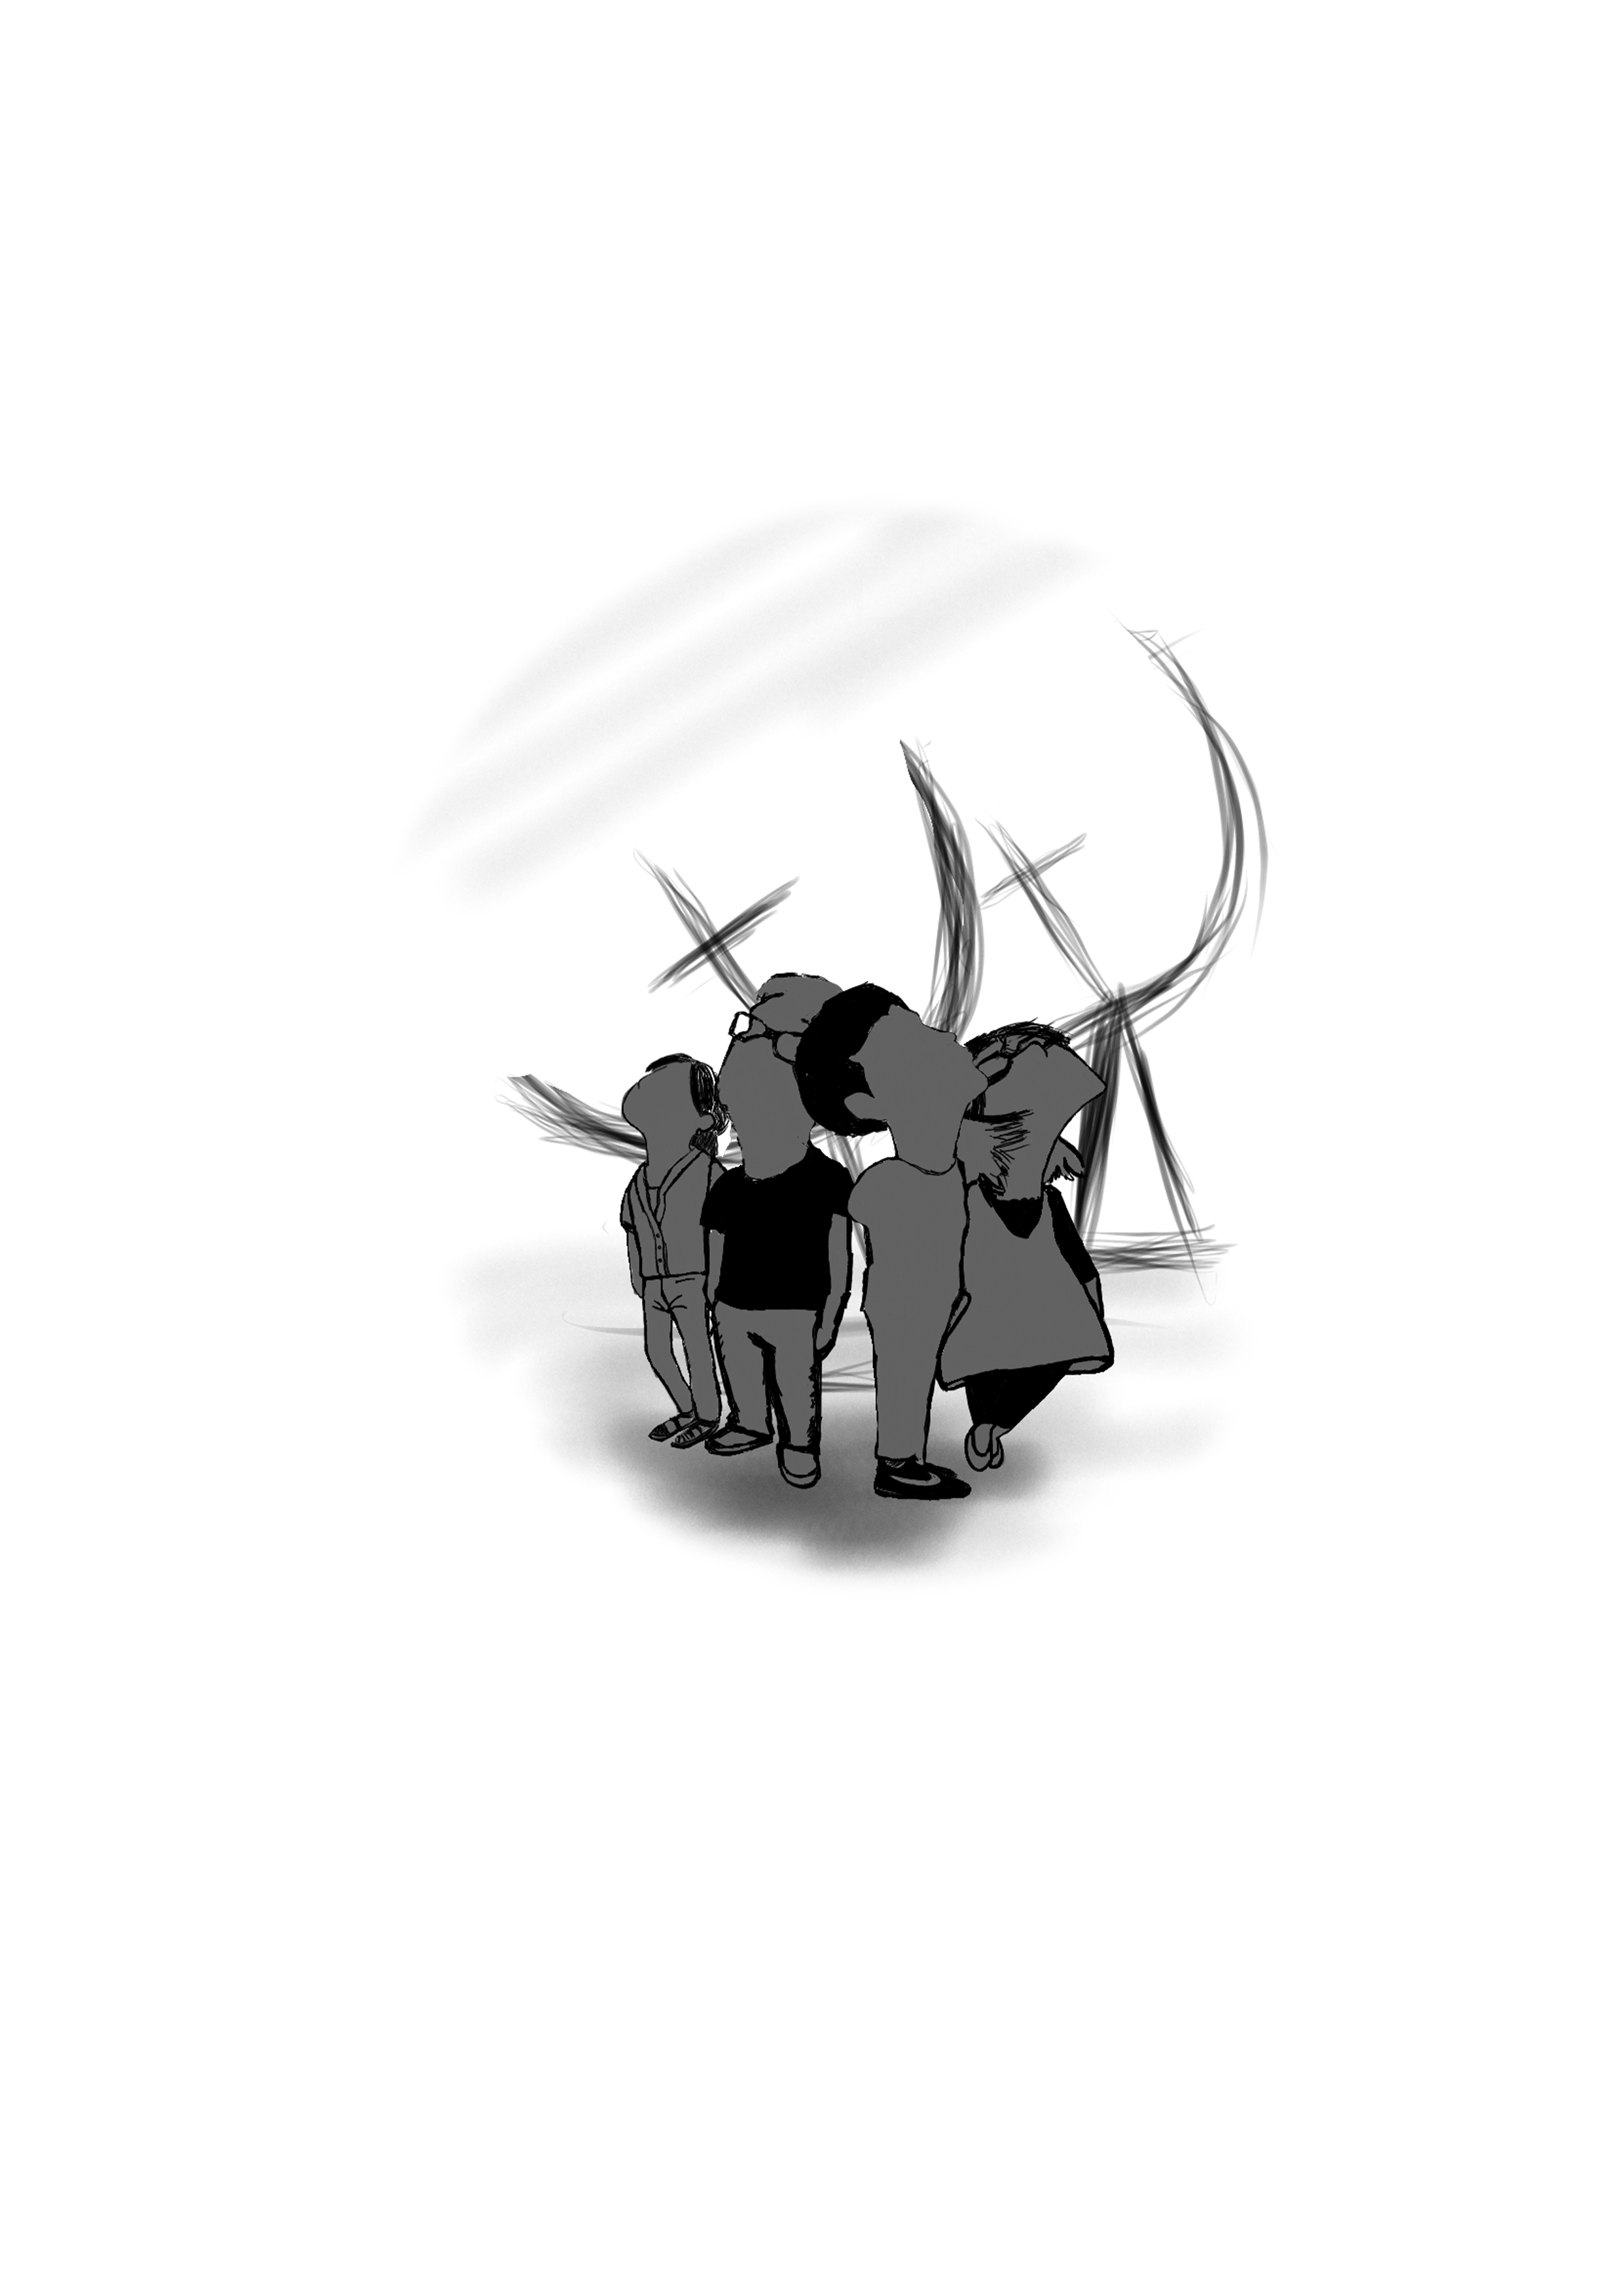
\includegraphics[width=21cm,height=29.7cm]{img/Cov}};
\begin{center}

\includegraphics[width=0.15\textwidth]{img/University-of-Mauritius-logo.png}~\\[1cm]

%\textsc{\Large Mini{-}project}\\[0.5cm]

% Title
\HRule \\[0.4cm]
{ \huge \bfseries Digital Systems for the MITRA \\[0.4cm] }
{ \LARGE \bfseries (GPU Computing) \\[0.4cm] }

\HRule \\[0.5cm]

{\Large Submitted by}\\[0.2cm]

{\LARGE \bfseries Ruben Anderson Louis \\[2.5cm]}

{\Large Project submitted in the partial fulfillment for the degree of}\\[0.5cm]

{\Large \bfseries BSc (Hons) Physics with Computing}\\[2.0cm]
 
% Author and supervisor
%\begin{minipage}{0.4\textwidth}
%\begin{flushleft} \large
%\emph{Author:}\\
%Ruben Anderson \textsc{Louis} (1210449)\\
%
%\end{flushleft}
%\end{minipage}
%\begin{minipage}{0.4\textwidth}
%\begin{flushright} \large
%\emph{Supervisor:} \\
%Dr Girish Kumar \textsc{Beeharry} \\
%\hfill
%\end{flushright}
%\end{minipage}



\textsc{\LARGE University of Mauritius}\\[0.2cm]
\textsc{\large  Faculty of Science}\\[0.2cm]
\textsc{\large Department of Physics}\\[0.5cm]
% Bottom of the page
{\Large Vers. 1.01 - \today} %For reviewing sake
%{\Large March, 2015}
\end{center}
\clearpage
\end{titlepage}




%% ----------------------------------------------------------------

\setstretch{1.3}  % It is better to have smaller font and larger line spacing than the other way round

% Define the page headers using the FancyHdr package and set up for one-sided printing
\fancyhead{}  % Clears all page headers and footers
\rhead{\thepage}  % Sets the right side header to show the page number
\lhead{}  % Clears the left side page header

\pagestyle{fancy}  % Finally, use the "fancy" page style to implement the FancyHdr headers

%% ----------------------------------------------------------------
% Declaration Page required for the Thesis, your institution may give you a different text to place here
\Declaration{

\addtocontents{toc}{\vspace{1em}}  % Add a gap in the Contents, for aesthetics

I, AUTHOR NAME, declare that this thesis titled, `THESIS TITLE' and the work presented in it are my own. I confirm that:

\begin{itemize} 
\item[\tiny{$\blacksquare$}] This work was done wholly or mainly while in candidature for a research degree at this University.
 
\item[\tiny{$\blacksquare$}] Where any part of this thesis has previously been submitted for a degree or any other qualification at this University or any other institution, this has been clearly stated.
 
\item[\tiny{$\blacksquare$}] Where I have consulted the published work of others, this is always clearly attributed.
 
\item[\tiny{$\blacksquare$}] Where I have quoted from the work of others, the source is always given. With the exception of such quotations, this thesis is entirely my own work.
 
\item[\tiny{$\blacksquare$}] I have acknowledged all main sources of help.
 
\item[\tiny{$\blacksquare$}] Where the thesis is based on work done by myself jointly with others, I have made clear exactly what was done by others and what I have contributed myself.
\\
\end{itemize}
 
 
Signed:\\
\rule[1em]{25em}{0.5pt}  % This prints a line for the signature
 
Date:\\
\rule[1em]{25em}{0.5pt}  % This prints a line to write the date
}
\clearpage  % Declaration ended, now start a new page
%% ----------------------------------------------------------------
% The "Funny Quote Page"
\pagestyle{empty}  % No headers or footers for the following pages

\null\vfill
% Now comes the "Funny Quote", written in italics
\textit{``An opening quote will be put here.''}

\begin{flushright}
The author's name will be there.
\end{flushright}

\vfill\vfill\vfill\vfill\vfill\vfill\null
\clearpage  % Funny Quote page ended, start a new page
%% ----------------------------------------------------------------
% The Abstract Page
%----------------------------------------------------------------------------------------
%	ABSTRACT PAGE
%----------------------------------------------------------------------------------------
\addtotoc{Abstract}  % Add the "Abstract" page entry to the Contents
\abstract{
\addtocontents{toc}{\vspace{1em}}  % Add a gap in the Contents, for aesthetics

In this report we give a brief account about imaging in the field of Radio Astronomy specifically on the technique coined Aperture Synthesis.
}
\clearpage  % Abstract ended, start a new page

%% ----------------------------------------------------------------
\setstretch{1.3}  % Reset the line-spacing to 1.3 for body text (if it has changed)
%----------------------------------------------------------------------------------------
%	ACKNOWLEDGEMENTS
%----------------------------------------------------------------------------------------
% The Acknowledgements page, for thanking everyone
\acknowledgements{\addtocontents{toc}{\vspace{1em}} % Add a gap in the Contents, for aesthetics
On the long road to the accomplishment of my undergraduate project and thesis I wish to acknowledge the following, first I am very grateful to my supervisor, Dr. G. K. Beeharry, for the opportunity he gave me to work on the topic, he has been an inspirational lecturer who encouraged me to pursue in the field of scientific computing, also most importantly I wish to thank him for his guidance, useful suggestions during the course of this project and his reviews, remarks and comments during the writing process of the thesis. I express my thanks to the lecturers of the Department of physics who during those 3 years here at the University of Mauritius contributed to build up the physicist I am today.

My special thanks goes to the MPhil student, Mr. Vinand Prayag, who was the first to trust me to work with him on the specific topic of software correlation, he was always there to talk and help when I needed advices, both on my project and my thesis.

I am also thankful to the technical staff of the Mauritius Radio Telescope and that of the department of physics for their help and guidance during the practical sessions and implementation of my project.

Extra credits goes to my classmates with whom we struggled with the BSc (Hons) Physics course, specially those of the computing branch who will recognise themselves, where the last two years together were a lot of fun and made my stay at the university a lot nicer.

I would also like to thank those closest to me for their support and my family who has always been behind me and helped me greatly to continue in the field of Physics at university level.

Last but not least as I am a faithful believer, and I believe that nothing happens without a reason I wish to thank God for everything, and making all of this possible whichever way it may have happened.
}

\clearpage % Start a new page

%% ----------------------------------------------------------------

\pagestyle{fancy}  %The page style headers have been "empty" all this time, now use the "fancy" headers as defined before to bring them back

%% ----------------------------------------------------------------
% TABLE OF CONTENS
\lhead{\emph{Contents}}  % Set the left side page header to "Contents"
\tableofcontents  % Write out the Table of Contents

%% ----------------------------------------------------------------
%Figures list
\lhead{\emph{List of Figures}}  % Set the left side page header to "List if Figures"
\listoffigures  % Write out the List of Figures

%% ----------------------------------------------------------------
%Tables list
%----------------------------------------------------------------------------------------
%	LIST OF CONTENTS/FIGURES/TABLES PAGES
%----------------------------------------------------------------------------------------
\lhead{\emph{List of Tables}}  % Set the left side page header to "List of Tables"
\listoftables  % Write out the List of Tables

%% ----------------------------------------------------------------
%Abbreviations list

%----------------------------------------------------------------------------------------
%	ABBREVIATIONS
%----------------------------------------------------------------------------------------

\clearpage % Start a new page

\setstretch{1.5} % Set the line spacing to 1.5, this makes the following tables easier to read

\lhead{\emph{Abbreviations}} % Set the left side page header to "Abbreviations"
\listofsymbols{ll} % Include a list of Abbreviations (a table of two columns)
{
\textbf{EM} & \textbf{E}lectro\textbf{m}agnetic \\
\textbf{FFT} & \textbf{F}ast \textbf{F}ourier \textbf{T}ransform \\
\textbf{GPU} & \textbf{G}raphics \textbf{P}rocessing \textbf{U}nit \\
\textbf{GPGPU} & \textbf{G}eneral \textbf{P}urpose \textbf{C}omputing on \textbf{G}raphics \textbf{P}rocessing \textbf{U}nits\\
\textbf{MEM} & \textbf{M}aximum \textbf{E}ntropy \textbf{M}ethod \\
\textbf{MITRA} & \textbf{M}ultifrequency \textbf{I}nterferometry \textbf{T}elescope for \textbf{R}adio \textbf{A}stronomy \\
\textbf{MRT} & \textbf{M}auritius \textbf{R}adio \textbf{T}elescope \\
\textbf{NNLS} & \textbf{n}on-\textbf{n}egative \textbf{l}east \textbf{s}quare \textbf{a}lgorithm \\
\textbf{R.A.} & \textbf{R}adio \textbf{A}stronomy \\
\textbf{SDR} & \textbf{S}oftware \textbf{D}efined \textbf{R}adio\\
\textbf{VLA} & \textbf{V}ery \textbf{L}arge \textbf{A}rray (Radiotelescope)\\
}

%% ----------------------------------------------------------------
% Physical Constants & Symbols
\clearpage  % Start a new page
\lhead{\emph{Physical Constants}}  % Set the left side page header to "Physical Constants"
\listofconstants{lrcl}  % Include a list of Physical Constants (a four column table)
{
% Constant Name & Symbol & = & Constant Value (with units) \\
Speed of Light & $c$ & $=$ & $2.997\ 924\ 58\times10^{8}\ \mbox{ms}^{-1}$ (exact)\\

}

%% ----------------------------------------------------------------
\clearpage  %Start a new page
\lhead{\emph{Symbols}}  % Set the left side page header to "Symbols"
\listofnomenclature{lll}  % Include a list of Symbols (a three column table)
{
% symbol & name & unit \\
$a$ & distance & m \\
$P$ & power & W (Js$^{-1}$) \\
& & \\ % Gap to separate the Roman symbols from the Greek
$\omega$ & angular frequency & rads$^{-1}$ \\
} 
%% ----------------------------------------------------------------
% End of the pre-able, contents and lists of things
% Begin the Dedication page

\setstretch{1.3}  % Return the line spacing back to 1.3
\pagestyle{empty}  % Page style needs to be empty for this page
\dedicatory{To my parents}

\addtocontents{toc}{\vspace{2em}}  % Add a gap in the Contents, for aesthetics


%% ----------------------------------------------------------------
\mainmatter	  % Begin normal, numeric (1,2,3...) page numbering
\pagestyle{fancy}  % Return the page headers back to the "fancy" style

% Include the chapters of the thesis, as separate files
% Just uncomment the lines as you write the chapters

%Version 1.01 @home 9:00 30.12.2014 
%Version notes:
%- Rough aims and objective added, cross reference to the appendix to git repository to be added.
%- Introduction on MITRA on the background of radio astronomy and imaging not yet added
%- Rough outline not yet done 
%%%%%%%%%%%%%%%%%%%%%%%%%%%%%%%%%%%%%%%%%%%%%%%%%%%%%%%%%%%%%%%%%%%%%%%%%%%%%%%%%%%%%%%%%%%%%%%%%%%%%
%%%%%%%%%%%%%%%%%%%%%%%%%%%%%%%%%%%%%%%%%%%%%%%%%%%%%%%%%%%%%%%%%%%%%%%%%%%%%%%%%%%%%%%%%%%%%%%%%%%%%
% Chapter 1

\chapter{Introduction} % Main chapter title

\label{Chapter1} % For referencing the chapter elsewhere, use \ref{Chapter1} 

\lhead{Chapter 1. \emph{Introduction}} % This is for the header on each page - perhaps a shortened title

%----------------------------------------------------------------------------------------

%----------------------------------------------------------------------------------------
\section{Digital Systems for the MITRA}
\label{sec:aboutDigiMITRA}
$\ldots$
\section{Aims and objectives}
\label{sec:aboutAimObjectives}
This project is aimed at the development, and testing of software and general purpose computing hardware for the Multi-frequency Interferometry for Astronomy (MITRA) array project. In so doing it will pave the way for a higher integration of digital systems as opposed to specialised hardware in the synthesis imaging process. The particular application which was focused on was that of high performance software correlation by the use of parallel computing. The central objective was to implement the DiFX (Distributed FX) software by Adam Deller for the MITRA by making it an off the shelf, user-friendly and custom documented software. The second part of the project was to explore the further possibilities opened up by General-purpose computing on Graphics Processing Units (GPGPU) to implement, develop, and test code taking advantage of its advance parallelism, and performance. I hope that the that the work on this particular project will not stay still and that this dissertation will inspire other people to continue to the work, thus from that initiative follows naturally the creation a public git repository:~\url{https://github.com/Benzy-Louis/MITRA_FX-CPU-GPU.git} where those interested to contribute to the project can continue the development, work on the source code, and improve the software and its documentation on their own or contribute for the same to the repository, those interested are freely encouraged to mail me at~\href{mailto:louis.ruben@gmail.com}{louis.ruben@gmail.com} if they want to contribute or have questions, suggestions on the project or on this dissertation and an appendix is written for the purpose of the use of the git repository $\ldots$

\
\section{Outline}
\label{sec:outline}
The dissertation is composed of $\ldots$ main chapters where $\ldots$ It is structured as follows \textit{chapter~\ref{Chapter1}} is an introduction to $\ldots$ Then \textit{chapter~\ref{litReview}} $\ldots$ % Introduction
\chapter{Literature Review}
\label{litReview}
\lhead{Chapter 2. \emph{Literature review}} % This is for the header on each page - perhaps a shortened title

%----------------------------------------------------------------------------------------
[Everything (codes,text, formatting) in this chapter is cheesy for the sake of having a quick overview while preparing the real literature review]
%----------------------------------------------------------------------------------------
\section{Mr. Vinand Prayag Lit. Rev. Plan advice}
\textbf{The past}\\
Hardware Correlator -> e.g. MRT room size, hardware $\ldots$\\
\textbf{Evolution}\\
Better processing power CPU made it feasible to replace hardware based system by software based ones. 
A rapid evolution of software defined radio (SDR). Direct applicability to radio astronomy.\\
\textbf{Examples}\\
Now we have what we call software telescopes such as the LOFAR powered by IBM supercomputers.\\
Recently SWINBURNE built a general purpose software correlator the DiFX,\\
\textbf{Pros. and cons. of DiFX.}


\section{[Cheesy] Prelimary gather up of abstract or similar}
\hfill\\
{\large 2008}\\ \nocite{jheengut2008MRTsoftcrr}
{\large Jheengut - Software Correlation}\\
\indent
\textit{Software correlation is seen to replace digital correlation as a step forward in removing the excessive cost for dedicated hardware in the near future. A software correlator for}
\noindent
{\large S. Ord, L. Greenhill, R. Wayth, D. Mitchell, K. Dale, H, Pfister, R. G. Edgar - GPUs  for data processing in the MWA}\\
\indent
\textit{The MWA is a next-generation radio interferometer under construction
in remote Western Australia. The data rate from the correlator makes
storing the raw data infeasible, so the data must be processed in real-time. The
processing task is of order 10 TFLOPs$^{-1}$. The remote location of the MWA
limits the power that can be allocated to computing. We describe the design and
implementation of elements of the MWA real-time data processing system which
leverage the computing abilities of modern graphics processing units (GPUs).
The matrix algebra and texture mapping capabilities of GPUs are well suited to
the majority of tasks involved in real-time calibration and imaging. Considerable
performance advantages over a conventional CPU-based reference implementation
are obtained.}
\hfill\\\\
{\large Chris Harris Karen Haines Lister Staveley-Smith - \hfill \\ GPU Accelerated Radio Astronomy Signal Convolution }\\
\indent
\textit{
The increasing array size of radio astronomy interferometers is causing the associated computation to scale quadratically with the number of array signals. Consequently, efficient usage of alternate processing architectures should be explored in order to meet this computational challenge. Affordable parallel processors have been made available to the general scientific community in the form of the commodity graphics card. This work investigates the use of the Graphics Processing Unit (GPU) in the parallelisation of the combined conjugate multiply and accumulation stage of a correlator for a radio astronomy array. Using NVIDIA’s Compute Unified Device Architecture, our testing shows processing speeds from one to two orders of magnitude faster than a Central Processing
Unit (CPU) approach.
}

\hfill\\\\
{\large Andrew Woods,
Michael Inggs and Alan Langman - \hfill \\ Accelerating a Software Radio Astronomy
Correlator using FPGA co-processors }

\textit{This article presents and characterises our work on
accelerating a software radio astronomy correlator
using reconfigurable computing (RC) hardware. Radio
astronomy correlation is an embarrassingly parallel signal
processing application, which is used heavily in
radio astronomy for imaging and other astronomical
measurements. Radio astronomy correlators typically
operate on huge data sets and often require real-time
processing, as storage of raw data is impractical - resulting
in substantial computational requirement. Currently
FPGAs are the preferred processing architecture used in
modern large radio astronomy correlators [1] and perform
well on the types of DSP functions that correlators
perform.
In this paper we set out to accelerate the DiFX
(Distributed FX) correlator, a software correlator, using
FPGA reconfigurable computing hardware. —– hoping
to inherit some of the advantages that larger production
FPGA correlators have over software.}\\

\noindent
{\large 2009}\\
\noindent
{\large NVIDIA - \hfill \\
NVIDIA’s Next Generation
CUDA$^{\textrm{TM}}$ Compute Architecture: Fermi$^{\textrm{TM}}$}\\
\noindent
{\large Adam Trevis Deller - \hfill \\ Precision VLBI astrometry: Instrumentation, algorithms and pulsar  parallax determination}

\textit{This thesis describes the development of DiFX, the first general–purpose software correlator for radio interferometry, and its use with the Australian Long Baseline Array to complete the largest Very Long Baseline Interferometry (VLBI) pulsar astrometry program undertaken to date in the Southern Hemisphere.This two year astrometry program has resulted in the measurement of seven new pulsar parallaxes, which has more than trebled the number of measured VLBI pulsar parallaxes in the Southern Hemisphere. These measurements included a determination of the distance and transverse velocity of PSR J0437–4715 with better than 1\% accuracy, enabling improved tests of General Relativity; the first significant measurement of parallax for the famous double pulsar system PSR J0737–3039A/B, which will allow tests of General Relativity in this system to proceed to the 0.01\% level and also offers insights into its formation and high–energy emission; and a factor of four revision to the estimated distance of PSR J0630–2834, which had previously appeared to possess extremely unusual x–ray emission characteristics. Additionally, the ensemble of refined distance and transverse velocity estimates have enabled a widely applicable improvement in knowledge of pulsar luminosities in several wavebands and the Galactic electron distribution at southern latitudes. Finally, the DiFX software correlator developed to enable this science has been extensively tested and verified against three existing hardware correlators, and is now an integral part of the upgraded Long Baseline Array Major National Research Facility used by astronomers throughout Australia and the world; furthermore, it has been selected to facilitate a major upgrade of the world’s only full–time VLBI instrument, the Very Long Baseline Array operated by the National Radio Astronomy Observatory in the US.
}\\
\noindent
{\large Rob V. van Nieuwpoort,
John W. Romein  - \hfill \\ Using Many-Core Hardware to Correlate
Radio Astronomy Signals }

\textit{A recent development in radio astronomy is to replace traditional
dishes with many small antennas. The signals are combined to form
one large, virtual telescope. The enormous data streams are crosscorrelated
to filter out noise. This is especially challenging, since
the computational demands grow quadratically with the number of
data streams. Moreover, the correlator is not only computationally
intensive, but also very I/O intensive. The LOFAR telescope, for
instance, will produce over 100 terabytes per day. The future SKA
telescope will even require in the order of exaflops, and petabits/s
of I/O. A recent trend is to correlate in software instead of dedicated
hardware. This is done to increase flexibility and to reduce
development efforts. Examples include e-VLBI and LOFAR.
In this paper, we evaluate the correlator algorithm on multi-core
CPUs and many-core architectures, such as NVIDIAand ATIGPUs,
and the Cell/B.E. The correlator is a streaming, real-time application,
and is much more I/O intensive than applications that are
typically implemented on many-core hardware today. We compare
with the LOFAR production correlator on an IBM Blue Gene/P supercomputer.
We investigate performance, power efficiency, and
programmability. We identify several important architectural problems
which cause architectures to perform suboptimally. Our findings
are applicable to data-intensive applications in general.
The results show that the processing power and memory bandwidth
of current GPUs are highly imbalanced for correlation purposes.
While the production correlator on the Blue Gene/P achieves a superb 96\% of the theoretical peak performance, this is only 14\%
on ATI GPUs, and 26\% on NVIDIA GPUs. The Cell/B.E. processor,
in contrast, achieves an excellent 92\%. We found that the
Cell/B.E. is also the most energy-efficient solution, it runs the correlator
5-7 times more energy efficiently than the Blue Gene/P. The
research presented is an important pathfinder for next-generation
telescopes.
}\\

\noindent
{\large 2010}\\
\noindent
{\large Andrew Woods,
Michael Inggs and Alan Langman - \hfill \\ Accelerating a Software Radio Astronomy
Correlator using FPGA co-processors }\\
\indent \textit{This thesis attempts to accelerate compute intensive sections of a frequency domain radio
astronomy correlator using dedicated co-processors. Two co-processor implementations were
made independently with one using reconfigurable hardware (Xilinx Virtex 4LX100) and the
other uses a graphics processor (Nvidia 9800GT). The objective of a radio astronomy correlator
is to compute the complex valued correlation products for each baseline which can be used
to reconstruct the sky’s radio brightness distribution. Radio astronomy correlators have huge
computation demands and this dissertation focuses on the computational aspects of correlation,
concentrating on the X-engine stage of the correlator.
Although correlation is an extremely compute intensive process, it does not necessarily require
custom hardware. This is especially true for older correlators or VLBI experiments, where
the processing and I/O requirements can be satisfied by commodity processors in software.
Discrete software co-processors like GPUs and FPGAs are an attractive option to accelerate
software correlation, potentially offering better FLOPS/watt and FLOPS/\$ performance.
In this dissertation we describe the acceleration of the X-engine stage of a correlator on a
CUDA GPU and an FPGA. We compare the co-processors’ performance with a CPU software
correlator implementation in a range of different benchmarks. Speedups of 7x and 12.5x were
achieved on the FPGA and GPU correlator implementations respectively.
Although both implementations achieved speedups and better power utilisation than the CPU
implementation, the GPU implementation produced better performance in a shorter development
time than the FPGA. The FPGA implementation was hampered by the development
tools and the slow PCI-X bus, which is used to communicate with the host. Additionally, the
Virtex 4 LX100 FPGA was released two years before the Nvidia G80 GPU and so is more behind
the current technologies. However, the FPGA does have an advantage in terms of power
efficiency, but power consumption is only a concern for large compute clusters. We found that
using GPUs was the better option to accelerate small-scale software X-engine correlation than
the Virtex 4 FPGA.
}\\

\noindent
{\large Nicolas PLATEL - Implémentation d’un corrélateur sur une carte GPU.  }\\
\indent \textit{Le but de ce projet est d’implémenter un corrélateur de type FX en Software sur une carte GPU de la marque NVIDIA. Ce corrélateur permettra aux étudiants de finir la construction du télescope étudié et obtenir des images du ciel. Il a pour but également de donner quelques notions sur Cuda aux étudiants le désirants. Dans le but d’étudier des phénomènes physiques connus et de valider mon projet, des résultats expérimentaux ont été effectués grâce aux antennes et au récepteur numérique créé précédemment. Enfin, une interface graphique a été créée pour faciliter l’utilisation du corrélateur à l’utilisateur.
}\\

\noindent
{\large Hobiger T., Kimura M., Takefuji K, Oyama T., Koyama Y., Kondo T., Gotoh T., Amagai J. \hfill \\ GPU based software correlators-perspectives for VLBI2010 }\\
\indent \textit{Caused by historical separation and driven by the requirements of the PC gaming 
industry, Graphics Processing Units (GPUs) have evolved to massive parallel processing 
systems which entered the area of non-graphic related applications. Although a single 
processing core on the GPU is much slower and provides less functionality than its 
counterpart on the CPU, the huge number of these small processing entities outperforms 
the classical processors when the application can be parallelized. Thus, in  
recent years various radio astronomical projects have started to make use of this 
technology either to realize the correlator on this platform or to establish the 
post-processing pipeline with GPUs. Therefore, the feasibility of GPUs as a choice 
for a VLBI correlator is being investigated, including pros and cons of this technology. 
Additionally, a GPU based software correlator will be reviewed with respect to 
energy consumption/GFlop/sec and cost/GFlop/sec. 
}\\

\noindent
{\large Patrick Brandt, Ron Duplain,
Paul Demorest, Randy McCullough, Scott
Ransom, Jason Ray \hfill \\ Heterogeneous real-time computing in radio astronomy  }\\
 \indent \textit{Modern computer architectures suited for general purpose computing are often not the best choice for either I/O-bound or compute-bound problems. Sometimes the best choice is not to choose a single architecture, but to take advantage of the best characteristics of different computer architectures to solve your problems. This paper examines the tradeoffs between using computer systems based on the ubiquitous X86 Central Processing Units (CPU's), Field Programmable Gate Array (FPGA) based signal processors, and Graphical Processing Units (GPU's). We will show how a heterogeneous system can be produced that blends the best of each of these technologies into a real-time signal processing system. FPGA's tightly coupled to analog-to-digital converters connect the instrument to the telescope and supply the first level of computing to the system. These FPGA's are coupled to other FPGA's to continue to provide highly efficient processing power. Data is then packaged up and shipped over fast networks to a cluster of general purpose computers equipped with GPU's, which are used for floating-point intensive computation. Finally, the data is handled by the CPU and written to disk, or further processed. Each of the elements in the system has been chosen for its specific characteristics and the role it can play in creating a system that does the most for the least, in terms of power, space, and money.
}\\


\noindent
{\large GINOURIE Sabera Bibi \hfill \\ A prototype front-end and back-end receiver system for radioastronomy }\\
\indent \textit{The first part of the project consisted of designing and building a front-end and back-end system for radioastronomy. Eight Log-periodic dipole antennas (available at the MRT) were used for the front-end.
In the second part, a new data acquisition card was used. This card was studied and programmed before used. The card was tested several times in order to check whether the analog data were digitised. Next, the whole system was tested and observations were carried out. Celestial objects like Virgo A and Centaurus A were successfully observed.
}\\

\noindent
{\large 2011}\\
\noindent
{\large V. K. Veligatla, P. Labropoulos, L. V. E. Koopmans - \hfill \\ Adaptive Beam-forming for Radio Astronomy On GPU }\\
\indent \textit{The LOFAR radio telescope consists of tens of thousands of dipole antennas that combine
their signals to operate as a single large radio telescope. The truly innovative aspect of
this new telescope is that its pointing system is not mechanical. It is steered by combining
the electric signals from different elements using advanced beam-forming software. Imaging
software is one of the important aspects of processing the high-volume data streams
produced by LOFAR, and is one of the best places to use GPUs to achieve processing
speed. We were able to achieve up to 30 times performance gain compared to the CPU
implementation in novel, computationally intensive techniques such as the Minimum Variance
Distortionless Response (MVDR). We have gained 5-6 times speed-up compared to
the CPU implementation for standard imaging algorithms.
}\\

\noindent
{\large M. A. Clark, P. C. La Plante, L. J. Greenhill - \hfill \\ Accelerating Radio Astronomy Cross-Correlation with Graphics Processing Units }\\
\indent \textit{We present a highly parallel implementation of the cross-correlation of time-series data using graphics processing units (GPUs), which is scalable to hundreds of independent inputs and suitable for the processing of signals from "Large-N" arrays of many radio antennas. The computational part of the algorithm, the X-engine, is implementated efficiently on Nvidia's Fermi architecture, sustaining up to 79\% of the peak single precision floating-point throughput. We compare performance obtained for hardware- and software-managed caches, observing significantly better performance for the latter. The high performance reported involves use of a multi-level data tiling strategy in memory and use of a pipelined algorithm with simultaneous computation and transfer of data from host to device memory. The speed of code development, flexibility, and low cost of the GPU implementations compared to ASIC and FPGA implementations have the potential to greatly shorten the cycle of correlator development and deployment, for cases where some power consumption penalty can be tolerated.
}\\

\noindent
{\large 2012}\\
\noindent
{\large NVIDIA - \hfill \\
NVIDIA’s Next Generation
CUDA$^{\textrm{TM}}$ Compute Architecture: Kepler$^{\textrm{TM}}$ GK110}\\

\noindent
{\large V. K. Veligatla, P. Labropoulos, L. V. E. Koopmans - \hfill \\ Adaptive Beam-forming for Radio Astronomy On GPU }\\
\indent \textit{The LOFAR radio telescope consists of tens of thousands of dipole antennas that combine
their signals to operate as a single large radio telescope. The truly innovative aspect of
this new telescope is that its pointing system is not mechanical. It is steered by combining
the electric signals from different elements using advanced beam-forming software. Imaging
software is one of the important aspects of processing the high-volume data streams
produced by LOFAR, and is one of the best places to use GPUs to achieve processing
speed. We were able to achieve up to 30 times performance gain compared to the CPU
implementation in novel, computationally intensive techniques such as the Minimum Variance
Distortionless Response (MVDR). We have gained 5-6 times speed-up compared to
the CPU implementation for standard imaging algorithms.
}\\

\noindent
{\large John W. Romein - \hfill \\ An Efficient Work-Distribution Strategy for Gridding Radio-Telescope Data on GPUs }\\
\indent \textit{This paper presents a novel work-distribution strategy for GPUs, that effciently convolves radio-telescope data onto a grid, one of the most time-consuming processing steps to
create a sky image. Unlike existing work-distribution strategies, this strategy keeps the number of device-memory accesses low, without incurring the overhead from sorting or searching within telescope data. Performance measurements show that the strategy is an order of magnitude faster than
existing accelerator-based gridders. We compare CUDA and OpenCL performance for multiple platforms. Also, we report very good multi-GPU scaling properties on a system with eight GPUs, and show that our prototype implementation is highly energy effcient. Finally, we describe how a unique property of GPUs, fast texture interpolation, can be used as a potential way to improve image quality.
}\\

\noindent
{\large Alessio Sclocco, Ana Lucia Varbanescu, Jan David Mol, Rob V. van Nieuwpoort - \hfill \\ Radio Astronomy Beam Forming on Many-Core Architectures }\\
\indent \textit{Traditional radio telescopes use large steel dishes
to observe radio sources. The largest radio telescope in
the world, LOFAR, uses tens of thousands of fixed, omnidirectional
antennas instead, a novel design that promises
ground-breaking research in astronomy. Where traditional telescopes
use custom-built hardware, LOFAR uses software to do
signal processing in real time. This leads to an instrument that
is inherently more flexible. However, the enormous data rates
and processing requirements (tens to hundreds of teraflops)
make this extremely challenging. The next-generation telescope,
the SKA, will require exaflops. Unlike traditional instruments,
LOFAR and SKA can observe in hundreds of directions
simultaneously, using beam forming. This is useful, for example,
to search the sky for pulsars (i.e. rapidly rotating highly
magnetized neutron stars). Beam forming is an important
technique in signal processing: it is also used in WIFI and 4G
cellular networks, radar systems, and health-care microwave
imaging instruments.
We propose the use of many-core architectures, such as 48-
core CPU systems and Graphics Processing Units (GPUs), to
accelerate beam forming. We use two different frameworks for
GPUs, CUDA and OpenCL, and present results for hardware
from different vendors (i.e. AMD and NVIDIA). Additionally,
we implement the LOFAR beam former on multi-core CPUs,
using OpenMP with SSE vector instructions. We use autotuning
to support different architectures and implementation
frameworks, achieving both platform and performance portability.
Finally, we compare our results with the production
implementation, written in assembly and running on an IBM
Blue Gene/P supercomputer. We compare both computational
and power efficiency, since power usage is one of the fundamental
challenges modern radio telescopes face. Compared to
the production implementation, our auto-tuned beam former
is 45–50 times faster on GPUs, and 2–8 times more power
efficient. Our experimental results lead to the conclusion that
GPUs are an attractive solution to accelerate beam forming.
}\\

\noindent
{\large V.Vamsi Krishna, Dr. Panos Labropoulos, Prof. Leon V.E. Koopmans  - \hfill \\ GPU's for Radio Imaging}\\
 \textit{- Signals from Sources (e.g. galaxies)\\
- Next Gen Antennas (e.g. LOFAR, SKA, ... )\\
- Image acquired after Processing (RFI elimination, Calibration).
}\\

\noindent
{\large Mike Clark with Lincoln Greenhill and Paul LaPlante - \hfill \\ Accelerating Radio Astronomy Cross-Correlation Beyond 1 Tflops Using Fermi }\\


\noindent
{\large 2013}\\
\noindent
{\large Dominique Ingala -Durban University of Technology \hfill \\ An Overview of the MITRA Radio Telescope
Signal Chain  }\\
\indent \textit{Project proposal: by Prof. Girish Beeharry\\
Locations: UoM and DUT\\
Operational frequency range: 200 – 800 MHz\\
Antenna type: Dual Polarized LPDA\\
2 arrays (8 LPDA’s per array)\\
Front-End RF and IF stage: Analog components\\
Digital Back-End: Software Defined Radio\\
Fiber optic links\\
Cost effective design
}\\

\noindent
{\large Harshavardhan Reddy Suda, Pradeep Kumar Gupta - \hfill \\ Powering Real-time Radio Astronomy Signal Processing with GPUs. Design of a GPU based real-time backend for the upgraded GMRT  }\\

\noindent
{\large Nitisha Pirthee - \hfill \\ Digital back end for MITRA prototype}\\
\indent \textit{In the first part of the project, USRP1 was used on GNU radio. A log periodic antenna was connected to one channel of the USRP and the expected peaks were observed. The second channel was not operational when tested. An array of sixteen channels was used as front end. A PCI-ADC card already available at MRT was used to do data acquisition. The program for data acquisition was improved. The card was tested several times and observations were carried out. Celestial objects like CAS A and Pictor A were successfully observed.
}\\

\noindent
{\large Harshavardhan Reddy Suda, Pradeep Kumar Gupta - \hfill \\ Powering Real-time Radio Astronomy Signal Processing with GPUs. Design of a GPU based real-time backend for the upgraded GMRT  }\\

\noindent
{\large Ben Barsdell, Mike Clark, Lincoln Greenhill, Jonathon Kocz - \hfill \\ ACCELERATING RADIO ASTRONOMY CROSS-CORRELATION USING THE KEPLER ARCHITECTURE  }\\
\indent \textit{Kepler GK110 optimisation
}\\

\noindent
{\large 2014}\\
\noindent
{\large Ben Barsdell, Mike Clark, Lincoln Greenhill, Jonathon Kocz - \hfill \\ PETASCALE CROSS-CORRELATION }\\

\noindent
{\large Amr H. Hassan, Christopher Fluke, David Barnes, Virginia Kilborn - \hfill \\ Astronomical “Big Data” Analysis and Visualization }\\

\noindent
{\large Alex Bogert, John Holdener, and Nicholas Smith - \hfill \\ Interactive Visualization of Astrophysical Data }\\
\indent \textit{Yt is an analysis and visualization system for astrophysical volumetric data
that is openly developed and freely available. At its core, yt provides a method of
describing physical rather than computational objects inside an astrophysical
simulation. yt provides methods for selecting regions, applying analysis to regions,
visualizing (including volume rendering, projections, slices, phase plots) and
exporting data to external analysis packages.
}\\

\noindent
{\large S. Bhatnagar,P. K. Gupta, M. Clark - \hfill \\ GPU based imager for radio astronomy }\\

\noindent
{\large Mario Guillaume CECILE - \hfill \\ Enhancement of some computational physics algorithms using Parallel Computing and the Graphical Processing Unit}\\
\indent \textit{Scientific computing has become an important method for testing and improving current scientific models and theories. Recent developments in computer architecture have helped to study more complex systems using High Performance Computing (HPC). In this project,Grain Growth simulation and the soft-sphere Discrete Element Method (DEM) are enhanced to be able to consider larger matrix sites in the Grain Growth simulation and a large number of particles in the DEM model. Parallel computing using Message Passing Interface (MPI) is used as well as CUDA for programming on the GPU. For the Grain Growth simulation, effects of foreign particles are investigated while for the DEM model, free-falling of particles in a packed bed is studied. The results presented in this work help to give further understanding about the physics involved behind both the Grain Growth and DEM. This work furthermore demonstrates how the use of parallel processing can helps scientists to enhance their code.
}\\

\noindent
{\large NVIDIA - \hfill \\
NVIDIA GeForce GTX 750 Ti
Featuring First-Generation Maxwell GPU Technology, Designed for Extreme Performance per Watt}

NVIDIA GeForce GTX 980
Featuring Maxwell, The Most Advanced GPU Ever Made. % Literature Review
% Chapter 3

\chapter{Synthesis Imaging} % Main chapter title

\label{Chapter3} % For referencing the chapter elsewhere, use \ref{Chapter3} 

\lhead{Chapter 3. \emph{Synthesis Imaging}} % This is for the header on each page - perhaps a shortened title

%----------------------------------------------------------------------------------------

%----------------------------------------------------------------------------------------
$\ldots$ % DiFX
% Chapter 3

\chapter{Distributed FX Correlation - The DiFX software} % Main chapter title

\label{Chapter4} % For referencing the chapter elsewhere, use \ref{Chapter3} 

\lhead{Chapter 4. \emph{Distributed FX Correlation - The DiFX software}} % This is for the header on each page - perhaps a shortened title

%----------------------------------------------------------------------------------------

%----------------------------------------------------------------------------------------
$\ldots$ \\
This work made use of the Swinburne University of Technology software correlator, developed as part of the Australian Major National Research Facilities Programme and operated under licence. % GPU Tiled memory access

%% Chapter 5
\chapter{GPGPU FX Correlation }
\label{Chapter5} % For referencing the chapter elsewhere, use \ref{Chapter4} 
\lhead{Chapter 5. \emph{GPGPU FX Correlation}} % This is for the header on each page - perhaps a shortened title
%----------------------------------------------------------------------------------------

%----------------------------------------------------------------------------------------
\section{The GPU}
$\ldots$
\section{The xGPU code}
$\ldots$ 
\subsection{Tiled Memory Tasking Algorithm} % Main chapter title
$\ldots$
 % Experiment 2

%\input{./Chapters/Chapter6} % Results and Discussion

%\input{./Chapters/Chapter7} % Conclusion
\chapter{Conclusions and future works}
\label{ConclusionOnDissertation}
\lhead{\emph{Conclusions and future works}} 
\section{Conclusions}
$\ldots$
\section{Future works}
$\ldots$
%% ----------------------------------------------------------------
% Now begin the Appendices, including them as separate files

\addtocontents{toc}{\vspace{2em}} % Add a gap in the Contents, for aesthetics

\appendix % Cue to tell LaTeX that the following 'chapters' are Appendices

% Appendix A

\chapter{Background, mathematical derivations}
\label{AppendixA}
\lhead{Appendix A. \emph{Background, Mathematical derivations}}

$\ldots$	% Appendix Title

% Appendix B

\chapter{DiFX - Custom documentation}
\label{AppendixB}
\lhead{Appendix B. \emph{DiFX - Custom documentation}}

\section{DiFX - Preliminary setup}
[Vague content just to fill in, following$\ldots$]\\
To install the diFX-2.3 software correlator do the following things,
\begin{enumerate}
\item Download the source of the software somewhere using the following command
\begin{verbatim}
svn co https://svn.atnf.csiro.au/difx/master_tags/DiFX-2.3
\end{verbatim}

\item Install IPP, i.e.
\begin{verbatim}
>> cd $IPP_PATH
>> chmod +x install.sh
>> ./install.sh
\end{verbatim}

\item Install PGPLOT, following the instructions of the following website:\\
\url{http://pendientedemigracion.ucm.es/info/Astrof/software/howto/howto-pgplot.html}\\
Do the following,
\begin{verbatim}
>> cd /usr/local/src
>> mv ~/Downloads/pgplot5.2.tar.gz .
>> tar zxvf pgplot5.2.tar.gz
>> mkdir /usr/local/pgplot
>> cd /usr/local/pgplot
>> cp /usr/local/src/pgplot/drivers.list 
>> /usr/local/src/pgplot/makemake
 /usr/local/src/pgplot linux g77_gcc_aout
\end{verbatim}

Edit the file makefile
\begin{verbatim}
>> sudo gedit makefile &
\end{verbatim}
Change
\begin{verbatim}
FCOMPL=g77
# to 
FCOMPL=gfortran
\end{verbatim}
Then save, and compile
\begin{verbatim}
>> make
>> make cpg
>> make clean
\end{verbatim}
Export the paths
\begin{verbatim}
>> export PGPLOT_DIR=/usr/local/pgplot
>> export PGPLOT_DEV=/Xserve
\end{verbatim}

\item Install OpenMPI also.

\item Then go back to install diFX-2.3, edit the setup.bash file,
\begin{verbatim}
>> cd $DIFX_ROOT
>> sudo gedit setup.bash &
\end{verbatim}
\item Change the following paths environment variables, an  example  here for my setup,
\begin{verbatim}
####### ROOT PATHS ##########################
export DIFXROOT=/home/ruben/Final_Year_Project/DiFX/DiFX-2.3
export DIFX_PREFIX=$DIFXROOT
export PGPLOTDIR=/usr/local/pgplot/
export IPPROOT=/opt/intel/ipp/bin/

####### COMPILER ############################
export MPICXX=/usr/local/bin/mpicxx

# ALSO UNCOMMENT THESE THINGS ALSO

####### PORTS FOR DIFXMESSAGE ###############
# Uncomment these to enable DIFX_MESSAGES
export DIFX_MESSAGE_GROUP=224.2.2.1
export DIFX_MESSAGE_PORT=50201
export DIFX_BINARY_GROUP=224.2.2.1
export DIFX_BINARY_PORT=50202

\end{verbatim}
\item use the geniepc script with input the path /opt/intel
\begin{verbatim}
$DIFXROOT/applications/difx_monitor
\end{verbatim} 



\item Then we can start the installation of DiFX-2.3, go back to the root folder of diFX, and do the following,
\begin{verbatim}
>> source setup.bash
>> ./install-difx
\end{verbatim}

\item Now for the preliminary tests I have not automated the scripts which would allow me to run diFX without having to send out preliminary parameters first. To be able to use the program one must set up the RPC. So the rpcbind package has to be installed.

\item To make rpcbind work,
\begin{verbatim}
>> sudo -i service portmap stop
>> sudo -i rpcbind -i -w
>> sudo -i service portmap start 
\end{verbatim}

Then we can start the calculation server and check it for the host,
\begin{verbatim}
>> startCalcServer
>> checkCalcServer 127.0.0.1
# Setting up the CALC_SERVER environment variable to the local host
>> export CALC_SERVER=127.0.0.1
\end{verbatim}

To see the processes, open another terminal go to the root directory of diFX, source setup.bash and then run

It will display the processes taking place in the calculation, I attached a text file with that info.
\begin{verbatim}
>> errormon2
\end{verbatim}

\item When all this is done, one can try the example files, for the RDV70 data,
\begin{verbatim}
>> vex2difx example.v2d
>> calcif2 example_1.calc
>> mpirun -np 8 mpifxcorr example_1.input
\end{verbatim}


\item When the correlation is done, you can get the FITS-LDI file from it in the following way,

\begin{verbatim}
>> difx2fits example_1.difx
\end{verbatim}


\end{enumerate}
    % Appendix Title

% Appendix C

\chapter{The Git repository}
\label{AppendixC}
\lhead{Appendix C. \emph{The Git repository}}

$\ldots$ % Appendix Title
% Appendix D

\chapter{Progress Log}
\label{AppendixD}
\lhead{Appendix D. \emph{Progress Log}}

$\ldots$
\addtocontents{toc}{\vspace{2em}}  % Add a gap in the Contents, for aesthetics

\backmatter

%% ----------------------------------------------------------------
\label{Bibliography}
\lhead{\emph{Bibliography}}  % Change the left side page header to "Bibliography"
\bibliographystyle{plainnat}  % Use the "unsrtnat" BibTeX style for formatting the Bibliography
\bibliography{Bibliography}  % The references (bibliography) information are stored in the file named "Bibliography.bib"

\end{document}  % The End
%% ----------------------------------------------------------------